\begin{frame}
 \frametitle{Plane from Three Points}

\begin{columns}
  \column{6cm}
  Three non-collinear points\\
   $P_0(\textbf{r}_0)$, $P_1(\textbf{r}_1)$, $P_2(\textbf{r}_2)$
  \column{6cm}
  Plane $\mathcal{P}$\\
   passing through $P_0$, $P_1$, and $P_2$.
\end{columns}

\begin{columns}
  \column{7cm}
  \only<2>{Passing through $P_0(\textbf{r}_0)$\\
  Parallel to \\
  $\textbf{u} = \textbf{P}_0\textbf{P}_1 = \textbf{r}_1 -\textbf{r}_0$\\
    $\textbf{v} = \textbf{P}_0\textbf{P}_2 = \textbf{r}_2-\textbf{r}_0$.\\
Normal $\textbf{n} = \textbf{u} \times \textbf{v} =
(\textbf{r}_1-\textbf{r}_0) \times (\textbf{r}_2-\textbf{r}_0)$  \\

\textcolor[rgb]{0.98,0.00,0.00}{Implicit vectorial equation}:
  $$(\textbf{r}-\textbf{r}_0) \cdot \textbf{n} = 0$$
  %
  $$\boxed{(\textbf{r}-\textbf{r}_0) \cdot [(\textbf{r}_1-\textbf{r}_0) \times (\textbf{r}_2-\textbf{r}_0)] = 0}$$
%
$$\text{Vol}(R(\textbf{P}_0\textbf{P}, \textbf{P}_0\textbf{P}_1, \textbf{P}_0\textbf{P}_2)) = 0$$
  }

 \only<3>{
 \textcolor[rgb]{0.98,0.00,0.00}{Implicit vectorial equation}:
  %
  $$(\textbf{r}-\textbf{r}_0) \cdot [(\textbf{r}_1-\textbf{r}_0) \times (\textbf{r}_2-\textbf{r}_0)] = 0$$

 $P_0(x_0,y_0,z_0)$, $P_1(x_1,y_1,z_1)$, $P_2(x_2,y_2,z_2)$:\\

$P(x,y,z)$ is on plane $\mathcal{P}$:\\
\medskip
\textcolor[rgb]{0.98,0.00,0.00}{Implicit scalar equation}:
%
$$\left| \begin{array}{ccc}
          x-x_0 & y-y_0 & z-z_0 \\
          x_1-x_0 & y_1-y_0 & z_1-z_0 \\
          x_2-x_0 & y_2-y_0 & z_2-z_0	
         \end{array}
\right| = 0\; .$$
%
  }

  \column{5.5cm}
    \begin{figure}
        \psfrag{O}{$O$}
        \psfrag{Pi}{$\mathcal{P}$}
        \psfrag{P}{$P$}
        \psfrag{P0}{$P_0$}
        \psfrag{P1}{$P_1$}
        \psfrag{P2}{$P_2$}
        \psfrag{r}{$\textbf{r}$}
        \psfrag{r0}{$\textbf{r}_0$}
        \psfrag{r1}{$\textbf{r}_1$}
        \psfrag{r2}{$\textbf{r}_2$}
        \psfrag{n}{$\textbf{n}$}
        \psfrag{u}{$\textbf{u}$}
        \psfrag{v}{$\textbf{v}$}
        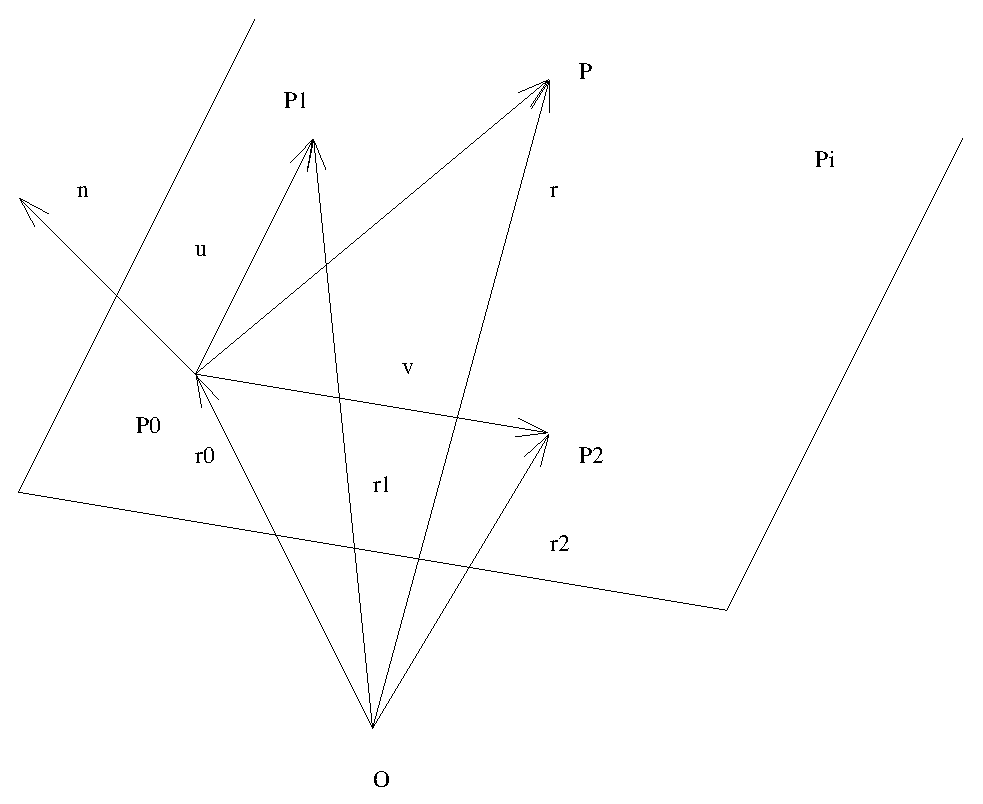
\includegraphics[height=2in]{../../modules/vectors/pictures/ok-plane_three_points.eps}
    \end{figure}
\end{columns}

\end{frame}

\begin{frame}
 \frametitle{Example}

$P_0(a,0,0)$, $P_1(0,b,0)$, $P_2(0,0,c)$ distinct points on axes.

$\mathcal{P}$: plane through $P_0$, $P_1$, $P_2$ = plane with given intercepts.

\bigskip

\begin{columns}
  \column{7cm}
  $\mathcal{P}$: parallel to \\
  $\textbf{P}_0\textbf{P}_1 = \langle -a, b, 0\rangle$,
    $\textbf{P}_0\textbf{P}_2 = \langle -a, 0 c\rangle$\\
    Normal to:
$\textbf{n} = \textbf{P}_0\textbf{P}_1 \times \textbf{P}_0\textbf{P}_2$
$$\textbf{n} =
\left| \begin{array}{ccc}
        \textbf{i} & \textbf{j} & \textbf{k} \\
	-a & b & 0 \\
        -a & 0 & c
       \end{array}
 \right| = bc \textbf{i} + ac \textbf{j} + ab \textbf{k}\; .$$
Implicit scalar equation of plane:
%
$$\langle x-a, y, z \rangle \cdot \langle bc, ac, ab \rangle = 0$$
%
$$bcx+acy + abz = abc \Longleftrightarrow \boxed{\frac{x}{a} + \frac{y}{b} + \frac{z}{c} = 1}$$
  \column{5.5cm}
     \begin{figure}
        \psfrag{O}{$O$}
        \psfrag{x}{$x$}
        \psfrag{y}{$y$}
        \psfrag{z}{$z$}
        \psfrag{A}{$P_0(a,0,0)$}
        \psfrag{B}{$P_1(0,b,0)$}
        \psfrag{C}{$P_2(0,0,c)$}
        \psfrag{n}{$\textbf{n}$}
        \psfrag{u}{$\textbf{u}$}
        \psfrag{v}{$\textbf{v}$}
        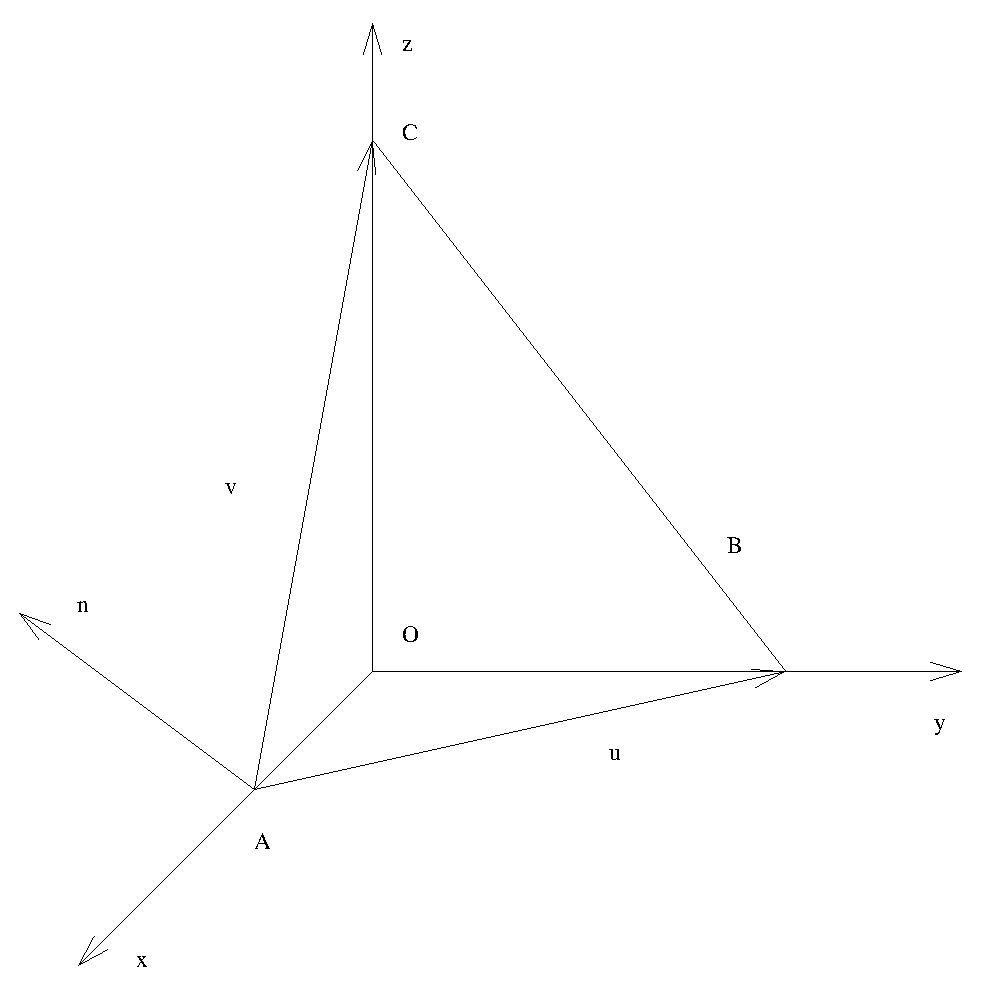
\includegraphics[width=2in]{../../modules/vectors/pictures/ok-plane_intercepts.eps}
    \end{figure}
\end{columns}
\end{frame}